\documentclass[a4,12pt]{article}
\usepackage[T1]{fontenc}
\usepackage{textcomp}
\usepackage[utf8]{inputenc}
\usepackage[english]{babel}
\usepackage{graphics}
\usepackage{graphicx}
\usepackage{epstopdf}
\usepackage{amsmath}
\usepackage{hyperref}
\usepackage{fancyvrb}
\usepackage{verbatim}
\usepackage{cmap}
%\renewcommand{\familydefault}{\sfdefault}
\textwidth=16cm
\oddsidemargin=0.1cm
\linespread{1.2}

\title{KernelGen -- multi-target accelerated kernels\linebreak generator for Fortran programs}
\author{Dmitry N. Mikushin\\ maemarcus@gmail.com}

\newcommand{\HRule}{\rule{\linewidth}{0.5mm}}
\DefineVerbatimEnvironment{code}{Verbatim}{frame=single, fontsize=\small}

\begin{document}

\maketitle

\begin{abstract}

KernelGen is open source-to-source translator with Fortran frontend, multiple backends (currently CUDA, OpenCL and CPU) and common runtime library. Fortran frontend extracts computational loops out of original source code, replacing them with calls to equivalent GPU or APU kernels. Additionally frontend can generate functions for per-kernel automatic results comparison between different implementations of the same loop. Runtime library handles both static (modules data, global variables) and dynamic (variables, fixed shape or allocatable arrays) kernel dependencies, automatically performing data load into device memory and fetching back the results. Runtime is designed thread-safe to provide seamless multi-GPU support for multithread and MPI applications. This article includes both simple test case for demonstration and real application study. To become production-ready prototype a couple of important device code optimization techniques must be implemented in KernelGen: tiling for shared memory utilization and loops interchanging.

\end{abstract}

\section{Motivation}

FF

\section{Code generator}

FF

\begin{figure}
\centering
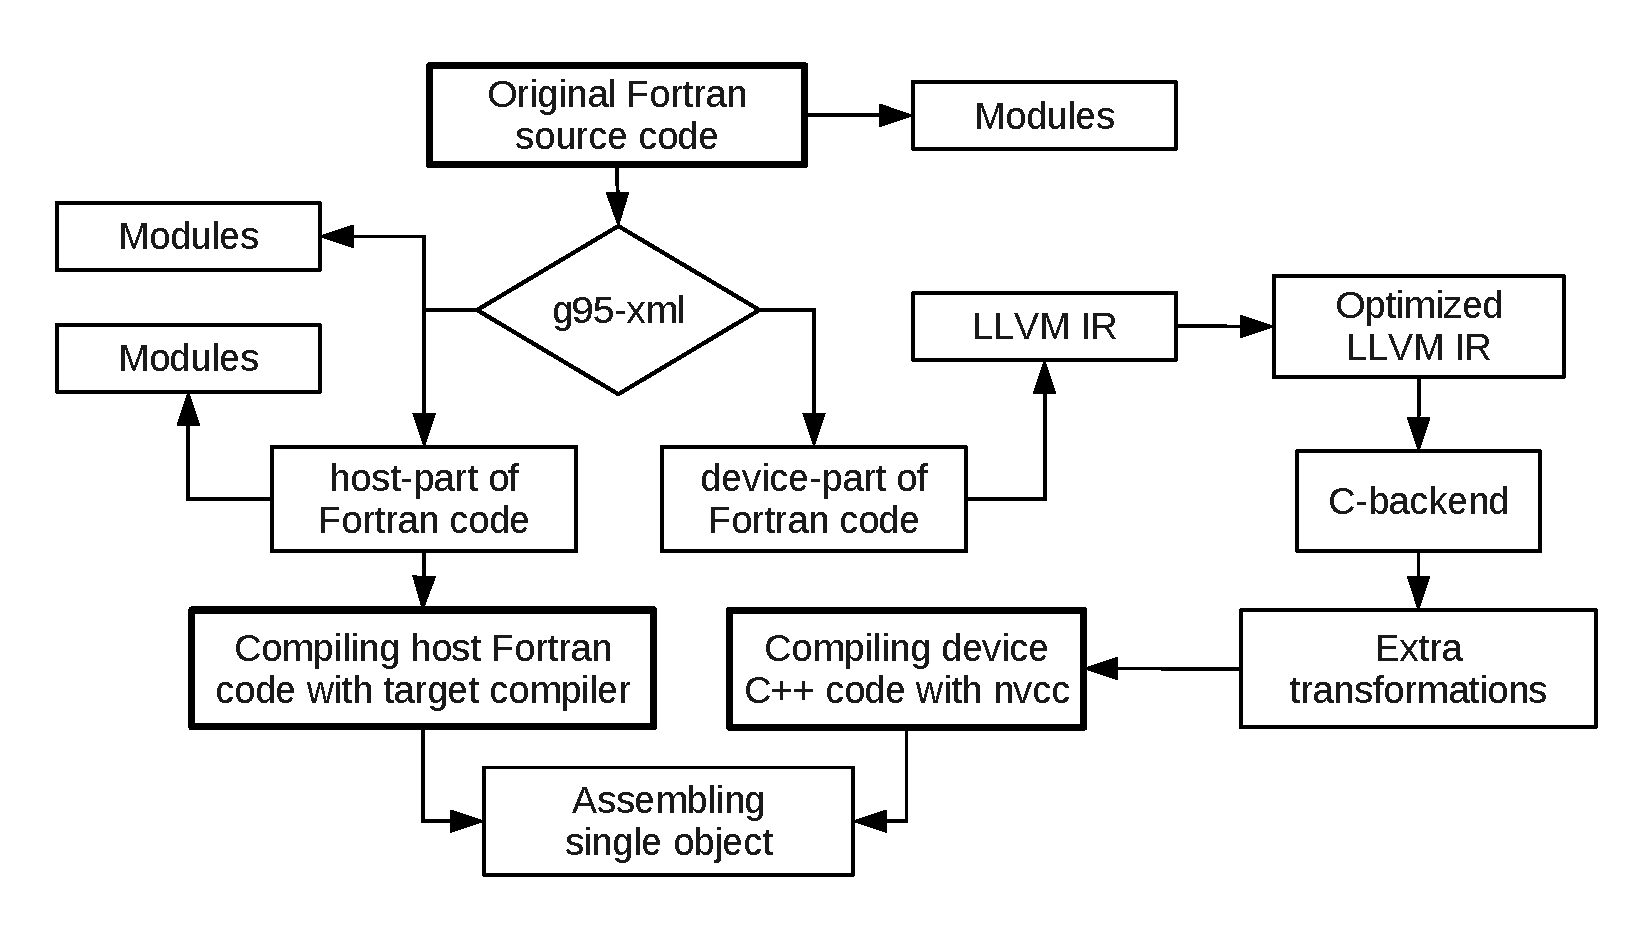
\includegraphics[scale=0.5]{figures/pipeline.pdf}
\caption{KernelGen code generation pipeline}
\label{fig:pipeline}
\end{figure}

\subsection{Kernels selection}

FF

\subsection{Backend}

FF

\section{Runtime library}

FF

\subsection{Multithreading and MPI support}

FF

\section{Examples}

FF

\section{Special features}

FF

\section{Conclusions}

FF

\section{Acknowledgments}

This work is a deep fusion of open-source software, business opportunities and scientific customers interests. With support and good will of Dr Gdaly Rivin and Dr Vladimir Krupchatnikov (Roshydromet, Russian Met Office) it became possible to start analyzing the needs of state-of-art weather forecasting models and build a comfortable tool specifically for scientific developers. Also with great support of various communities it became possible to reach the present state from ground level with minimum resources just in 5 months. I'd like to thank Roshydromet fellows Artem Petrov for coordination, testing and development, Dr Yulia Martynova for testing KernelGen with WRF model. I'm grateful to Sergey Kovylov of NVIDIA for constant support, Philippe Marguinaud of Meteo France for discussions and bug fixes in g95xml, Alexander Myltsev for testing and polishing build process, LLVM developers and specially Duncan Sands for discussions and bug fixes in C backend, GFortran team and specially Dr Tobias Burnus for Fortran consults and suggestions, Polly/LLVM team and specially Tobias Grosser for intensive discussions on optimizations related to polyhedral analysis. Thanks to Christopher Bergström of Pathscale for discussions and criticism.

\begin{figure}
\centering
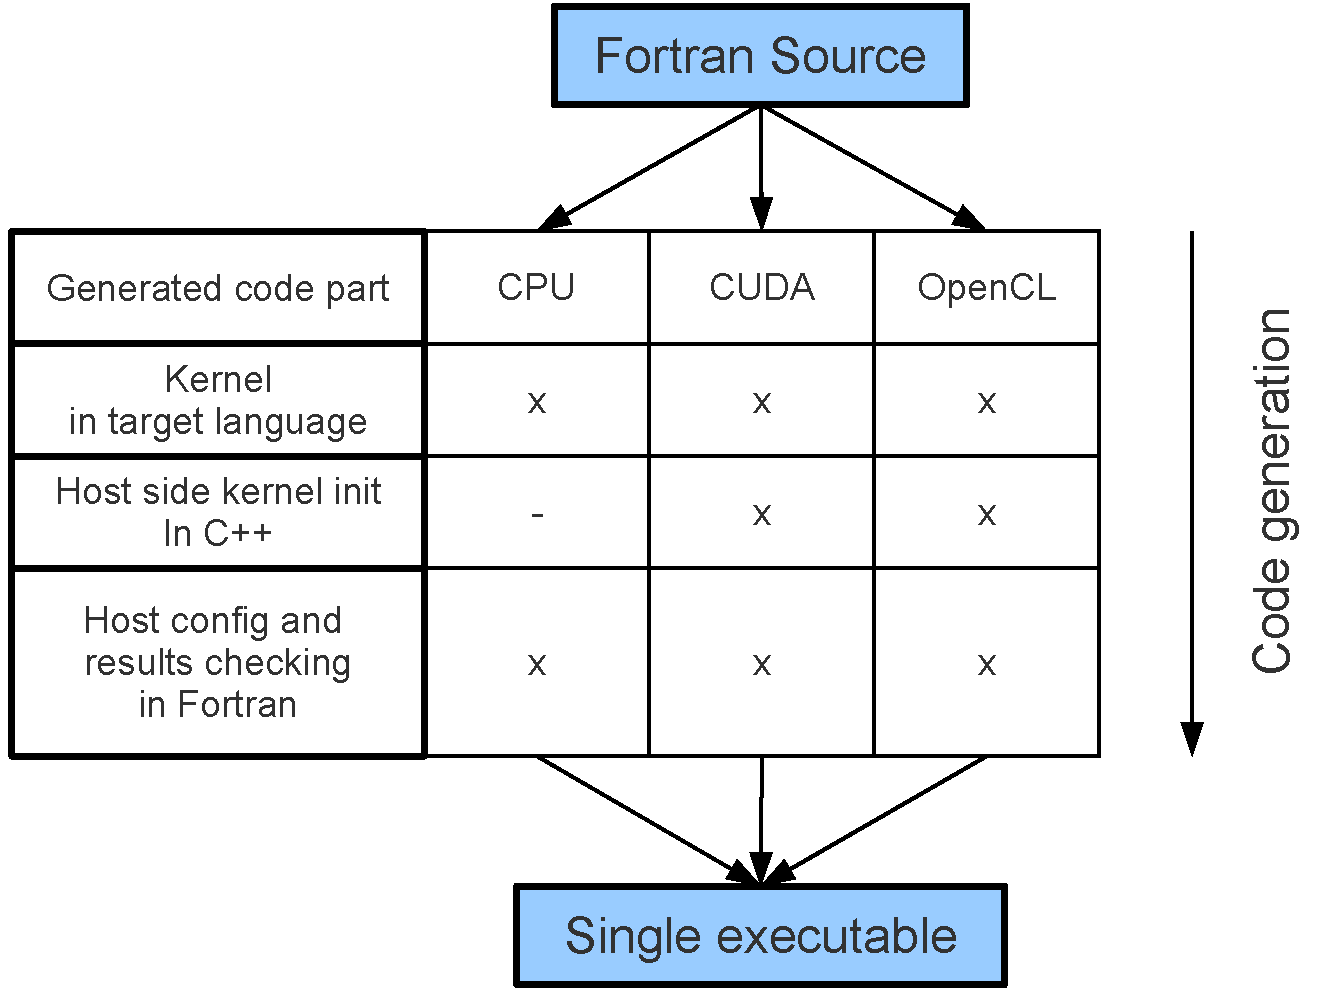
\includegraphics[scale=0.5]{figures/portability.pdf}
\caption{Multiple targets support in a single executable.}
\label{fig:portability}
\end{figure}

\begin{figure}
\centering
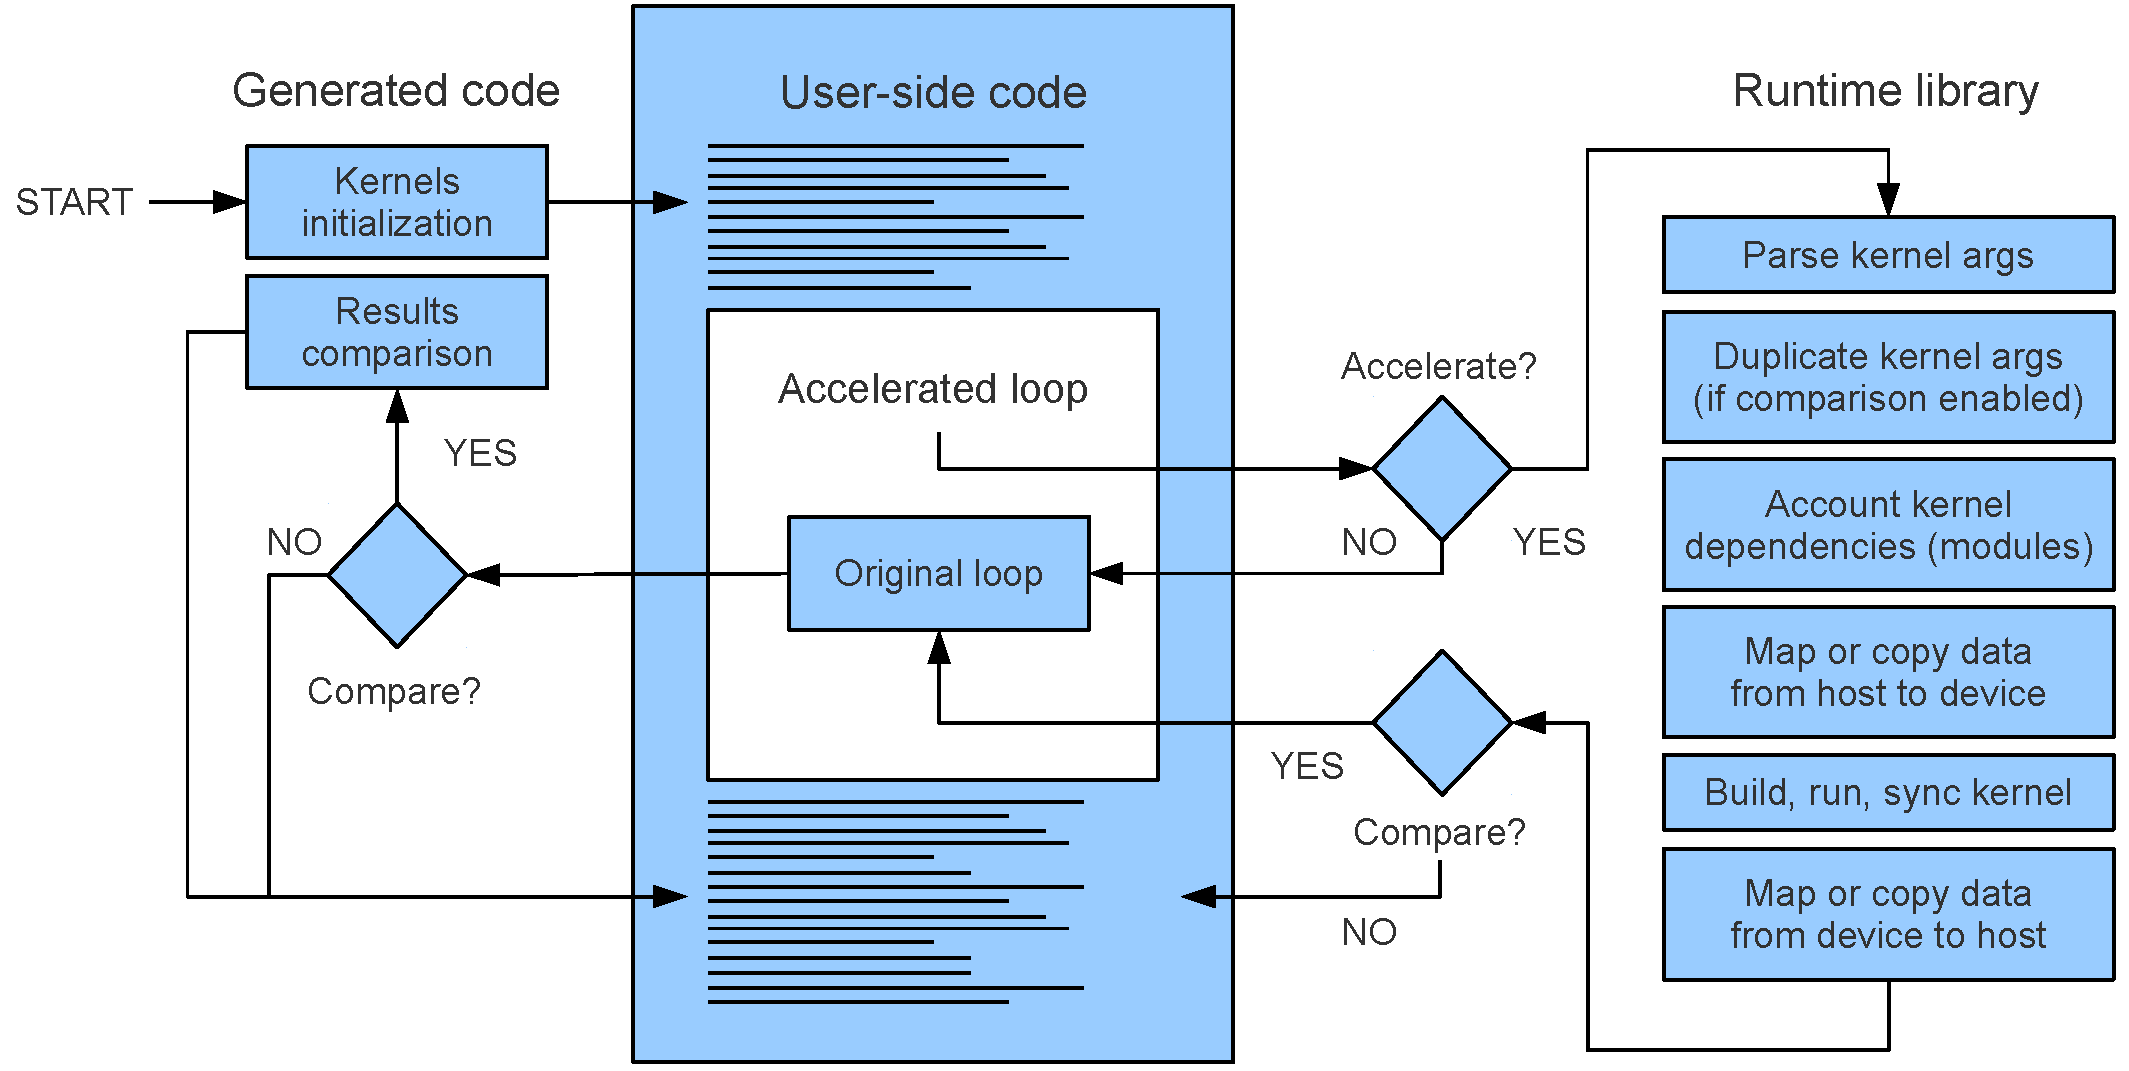
\includegraphics[scale=0.4]{figures/execution.pdf}
\caption{Execution model}
\label{fig:execution}
\end{figure}

\end{document}
